\documentclass{article}

\usepackage[a4paper, left=1.5cm, right=1.5cm, top=2cm, bottom=2cm]{geometry}

\usepackage{../../../../components/components}
\usepackage{hyperref}
\usepackage{fancyhdr}


% Configuration des en-têtes et pieds de page
\pagestyle{fancy}
\fancyhf{} % reset tout

\fancyhead[L]{DL2 Math-Info ASF4}
\fancyhead[C]{Algèbre}
\fancyhead[R]{2025-2026}

\fancyfoot[L]{Ewen Rodrigues de Oliveira}
\fancyfoot[R]{\thepage}

\begin{document}

\docTitle{Chapitre 6 : Endomorphismes des espaces euclidiens}

\section{Représentation matricielle d'un endomorphisme dans une base orthonormée}

\theorem{Proposition}{}{false}{
    Soit $E$ un espace euclidien. Soit $B = (e_1, e_2, \ldots, e_n)$ une base orthonormée de $E$.\\
    Soit $f \in \mathcal{L}(E)$ un endomorphisme de $E$. Alors :
    \[(Mat_B(f))_{ij} = \langle f(e_j), e_i \rangle \; \text{ pour tout } i, j \in \{1, 2, \ldots, n\}.\]
}

\noindent{\textbf{Démonstration :}\\
    $M_{ij} =$ i-ème coordonnée dans $B$ de $f(e_j)$ = $\langle f(e_j), e_i \rangle$ (car $B$ est orthonormée).
}

\section{Applications adjointes}

\subsection{Définition de l'adjoint}
\textit{La notion d'application adjointe est liée à celle d'application transposée, en utilisant l'isomorphisme naturel entre un espace vectoriel et son dual dans un espace euclidien.}

\theorem{Proposition}{}{false}{
    Soient $E, F$ deux espaces euclidiens et $u : E \to F$ une application linéaire.\\
    Alors $\exists ! v \in \mathcal{L}(F, E)$ telle que $\forall x \in E, \forall y \in F, \langle u(x), y \rangle_F = \langle x, v(y) \rangle_E$.
}
\vocabulary{On appelle $v$ l'\textbf{application adjointe} de $u$ et on la note $v = u^*$.}
\ndlr{cf. Laurent pour la preuve}

\reminder{Toute forme linéaire $\varphi$ sur un espace euclidien $E$ admet un unique $y \in E$ tel que $\forall x \in E \varphi = \langle \cdot, y \rangle$.\\
Plus particulièrement, l'application $y \to (x \to \langle x,y\rangle)$ est un isomorphisme.
}

\remark{On peut identifier $u^*$ à une application transposée $u^t : F^* \to E^*$, et ainsi $u^* = u^t$ via les isomorphismes naturels entre $E$ et $E^*$, et entre $F$ et $F^*$.


\begin{center}
    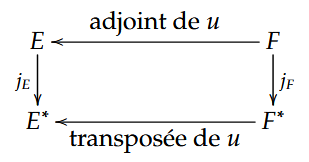
\includegraphics[width=0.25\textwidth]{./images/identification.png}
    \captionof{figure}{Schéma d'identification de $u^*$ à $u^t$ via les isomorphismes naturels entre $E$ et $E^*$, et entre $F$ et $F^*$.}
\end{center}
}

\theorem{Proposition}{Composition}{false}{
    Soient $E, F, G$ trois espaces euclidiens et $u : E \to F$, $v : F \to G$ deux applications linéaires.\\
    Alors $(v \circ u)^* = u^* \circ v^*$.
}

\subsection{Représentation matricielle de l'adjoint}

\theorem{Proposition}{}{false}{
    Soient $E,F$ deux espaces euclidiens munis de bases orthonormées $B_E$ et $B_F$ respectivement. Soit $u \in \mathcal{L}(E, F)$ et $u^* \in \mathcal{L}(F, E)$ son adjoint.\\
    Alors $Mat_{B_E, B_F}(u) = { }^t Mat_{B_F, B_E}(u^*)$.
}

\attention{Ce résultat n'est pas vrai si la base n'est pas orthonormée.}

\subsection{Endomorphismes autoadjoints}

\definition{
    Soit $E$ un espace euclidien. Un endomorphisme $u \in \mathcal{L}(E)$ est dit \textbf{autoadjoint} si $u = u^*$.
}

\theorem{Proposition}{Caractérisation}{false}{
    Soit $E$ un espace euclidien.\\
    Un endomorphisme $u \in \mathcal{L}(E)$ est autoadjoint si et seulement si, dans toute base orthonormée de $E$, la matrice de $u$ est symétrique.
}

\theorem{Proposition}{Stabilité du supplémentaire orthogonal}{false}{
    Soit $E$ un espace euclidien et $F$ un sous-espace vectoriel de $E$ stable par $u \in \mathcal{L}(E)$ autoadjoint.\\
    Alors $F^\perp$ est stable par $u$.\\
}

\remark{Considérons une matrice carrée symétrique $M$ de taille $n \times n$. Alors, en munissant $\mathbb{R}^n$ de son produit scalaire usuel, la matrice $M$ représente un endomorphisme auto-adjoint.}

\section{Isométries dans un espace euclidien}

\subsection{Définition}
\definition{
    Soit $E$ un espace euclidien. Un endomorphisme $u \in \mathcal{L}(E)$ est une \textbf{isométrie} si $\forall x, y \in E, \langle u(x), u(y) \rangle = \langle x, y \rangle$.
}

\remark{Si $f$ est une isométrie, alors $f$ est injective. Et comme un espace euclidien est de dimension finie, $f$ est bijective. Cette définition est donc un cas particulier ($E = F$) de celle énoncée dans le chapitre 4.}

\theorem{Proposition}{}{false}{
    Soit $E$ un espace euclidien, et soit $f \in \mathcal{L}(E)$. Alors les propriétés suivantes sont équivalentes :
    \begin{itemize}
        \item $f$ est une isométrie ;
        \item $f$ conserve le produit scalaire, \textit{i.e.} $\forall x, y \in E, \langle f(x), f(y) \rangle = \langle x, y \rangle$ ;
        \item $f$ envoie une base orthonormée de $E$ sur une base orthonormée de $E$ ;
        \item $f$ envoie toute base orthonormée de $E$ sur une base orthonormée de $E$.
    \end{itemize}
}
\newpage
\subsection{Groupes des isométries}

L'ensemble des isométries de $E$, un espace euclidien, forme un groupe pour la composition, appelé le \textbf{groupe orthogonal} de $E$ et noté $O(E)$.\\\\
\theorem{Proposition}{}{false}{
    Soit $E$ un espace euclidien.\\
    Toute isométrie de $E$ est un isomorphisme de $E$ et son inverse est également une isométrie. De plus, la composition de deux isométries est une isométrie.
}

\example{Rotations dans $\mathbb{R}^2$. Soit $r$ la rotation d'angle $\theta$ dans le plan euclidien $\mathbb{R}^2$, dont la matrice dans la base canonique est :
\[
    R_\theta = \begin{pmatrix}
        \cos \theta & -\sin \theta \\
        \sin \theta & \cos \theta
    \end{pmatrix}.
\]
Alors $R_\theta$ est une isométrie. Montrons-le directement en montrant que $R_\theta$ conserve la norme :\\
$\| R_\theta(\begin{pmatrix}
    x \\
    y
\end{pmatrix}) \|^2 = \| \begin{pmatrix}
    x \cdot \cos \theta - y \cdot \sin \theta \\
    x \cdot \sin \theta + y \cdot \cos \theta
\end{pmatrix} \|^2 = (x \cdot \cos \theta - y \cdot \sin \theta)^2 + (x \cdot \sin \theta + y \cdot \cos \theta)^2 = x^2 + y^2 = \| \begin{pmatrix}
    x \\
    y
\end{pmatrix} \|^2$.\\

\noindent De manière alternative, on remarquera que l'image par $R_\theta$ de la base canonique de $\mathbb{R}^2$ est une base orthonormée, ce qui montre que $R_\theta$ est une isométrie.
}

\subsection{Représentation matricielle}

\definition{
    Une matrice carrée $M$ de taille $n$ est \textbf{orthogonale} si les colonnes de $M$ forment une famille orthonormée pour le produit scalaire canonique de $\mathbb{R}^n$
}

\example{La matrice de la rotation d'angle $\theta$ dans la base canonique de $\mathbb{R}^2$ est orthogonale, car ses colonnes forment une famille orthonormée.}

\theorem{Théorème}{Caractérisation matricielle des isométries}{false}{
    Soit $E$ un espace euclidien muni d'une base orthonormée $e$. Soit $u \in \mathcal{L}(E)$. On a :
    \[
        u \text{ est une isométrie } \Leftrightarrow Mat_e(u) \text{ est orthogonale.}
    \]
}

\subsection{Adjoint d'une isométrie}

\theorem{Proposition}{}{false}{
    Soit $E$ un espace euclidien. $u \in \mathcal{L}(E)$ une isométrie si et seulement si $u^* = u^{-1}$.
}

\theorem{Corollaire}{}{false}{
    Une matrice $M$ est orthogonale si et seulement si ${}^t M \cdot M = I_n$.
}

\example{La matrice de la rotation d'angle $\theta$ dans la base canonique de $\mathbb{R}^2$ est orthogonale, et son inverse est la rotation d'angle $-\theta$, qui est également son adjoint.}

\subsection{Valeurs propres et déterminants des isométries}

\theorem{Proposition}{}{false}{
    Soit $E$ un espace euclidien, et soit $u \in \mathcal{L}(E)$ une isométrie de $E$.\\
    Alors ses seules valeurs propres possibles sont $\pm 1$ et on a $det(u) = \pm 1$.
}

\vocabulary{Les vecteurs propres associés à la valeur propre $1$ sont appelés \textbf{points fixes} de $u$.}

\definition{
    Soit $E$ un espace euclidien, et soit $F \subset E$ un sous-espace vectoriel.\\
    Considérons $p$ la projection orthogonale sur $F$. La \textbf{symétrie orthogonale} par rapport à $F$ est l'endomorphisme $s \in \mathcal{L}(E)$ défini par :
    \[
        s(x) = 2p(x) - x.
    \]
    Si $F$ est un hyperplan de $E$, alors $s$ est appelée une \textbf{réflexion}.

}

\end{document}